\chapter{Automatisation du processus d'investigation}
\label{Automatisation du processus d'investigation}
\thispagestyle{fancy}
Lorsqu'une \emph{error name} est révélée durant le Filtering test, de nombreuses données sont enregistrées dans un fichier journal (que l'on retrouve plus souvent sous le terme anglais de fichier "log".) Une analyse poussée de ces informations permet de déterminer la \emph{root cause} liée à l'\emph{error name} (partie \ref{Introduction:Expression du besoin:Hiérarchisation des erreurs}). Afin d'automatiser ce processus d'analyse, on s'appuie sur l'utilisation d'algorithmes d'apprentissage automatique. 

\section{Architecture High Level du système proposé}
\label{Automatisation du processus d'investigation: Achitecture High Level du système proposé}
L'architecture haut niveau de la solution que l'on propose est composée de deux couches: une couche \emph{root cause} et une couche \emph{error name}.
\begin{description}
	\item [Couche root cause] La couche \emph{root cause} permet de détecter la présence d'une \emph{root cause} dans le fichier log que l'on analyse. Il s'agit d'un algorithme d'apprentissage automatique entraîné à effectuer cette tâche.
	\item [Couche error name] La couche \emph{error name} est constituée d'un ensemble de couches \emph{root cause} de telle manière que lorsqu'un fichier log est mis en entrée du système, l'ensemble des couches \emph{root cause} sont activées. Ainsi, le système recherche la présence de chaque \emph{root cause} connue dans l'exemple étudié. On dit que les \emph{root causes} sont liées à l'\emph{error name}. On obtient en sortie de la couche \emph{error name} le nom de la \emph{root cause} ayant la plus forte probabilité d'avoir été reconnue.
\end{description} 

\subsubsection{Exemple de mise en place  d'une couche error name et de ses couches root cause}
\label{Automatisation du processus d'investigation: Achitecture High Level du système proposé: Exemple de mise en place  d'une couche error name et de ses couches root cause}
Afin d'exposer de manière concrète le fonctionnement de l'architecture haut niveau de la solution proposée, on soumet un exemple de mise en place d'une architecture de détection et son utilisation. \\

\paragraph{Mise en place du système de détection d'une root cause}
On souhaite dans un premier temps mettre en place l'architecture permettant de détecter la cause (\emph{root cause}) ayant entrainé la chute du robot lors du Filtering test (\emph{error name}). Cette étape consiste à créer les couches \emph{root cause}, i.e. entrainer différents algorithmes d'apprentissage automatique à reconnaître la \emph{root cause} pour laquelle ils ont été créés (figure \ref{fig:Creation des couches root cause}). Afin d'entraîner ces couches, on utilise les données utiles à chaque \emph{root cause}, contenues dans le fichier log généré lors de la chute d'un robot durant le Filtering Test. Par exemple, dans le cas de la \emph{root cause} "frottement des freins de la hanche", on utilisera les données "valeurs du senseur de la hanche" et "valeurs de l'actuateur de la hanche". Ces deux éléments correspondent aux features de notre système d'apprentissage (c.f. partie \ref{Le Machine Learning: Généralités sur le Machine Learning: Définition et principe général:Lexique}). L'ensemble de ces couches \emph{root cause} sont liées une couche \emph{error name}, ici la chute d'un robot.

\begin{figure}[h]
	\centering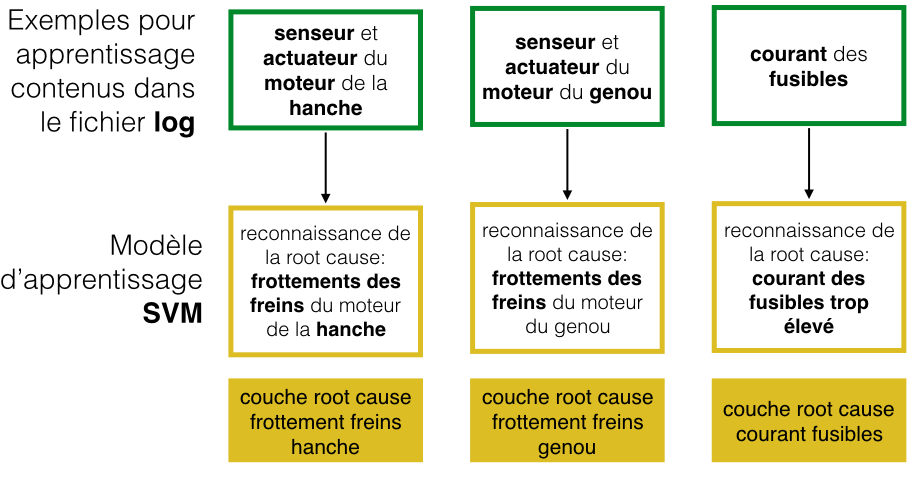
\includegraphics[height=7cm]{images/synoptique_root.png}
	\caption[Création des couches root cause]{Synoptique haut niveau de la création des couches \emph{root cause}. Les couches \emph{root cause} correspondent à des algorithmes d'apprentissage automatique que l'on entraîne à détecter la \emph{root cause} à laquelle ils sont associés. Par exemple, créer la couche \emph{root cause} "frottement du frein de la hanche" revient à entraîner un algorithme d'apprentissage de type SVM, à partir des valeurs senseurs et actuateurs de la hanche des fichiers logs.}
	\label{fig:Creation des couches root cause}
\end{figure}

